\chapter{\difficult{Model theory}}\label{chapter:model_theory}

    General references for this chapter are \cite{riehl_model, hovey}. For more on monoidal model categories see \cite{riehl_monoidal}. A good reference for the section on simplicial spaces and, in particular, the theory of Segal spaces is \cite{rezk}. For more on Reedy model structures see \cite{riehl_verity_reedy}. A gentle introduction to the theory of homotopy (co)limits can be found in \cite{lambrechts, hocolim_riehl}.

\section{Simplicial sets}

    \newdef{Simplex category}{\index{simplex!category}\label{model:simplex_category}
        \nomenclature[S_simpcat]{$\simplex$}{simplex category}
        The simplex category $\simplex$ has as objects the posets of the form $[n]:=\{0<\ldots<n\}$ and as morphisms the order-preserving maps.
    }
    \newdef{Simplicial set}{\index{simplicial!set}\label{model:simplicial set}
        The category $\mathbf{sSet}$ of simplicial sets is defined as the presheaf category $\mathbf{Psh}(\simplex)$. For all $n\in\mathbb{N}$ the set of \textbf{$n$-simplices in} $X$ is defined as the set $X_n:=X([n])$.
    }
    \newdef{Simplicial object}{\index{simplicial!object}\label{model:simplicial_object}
        By internalizing the notion of a simplicial set, one obtains the definition of a simplicial object, i.e.~a simplicial object in a category $\mathbf{C}$ is a $\mathbf{C}$-valued presheaf on $\simplex$.
    }
    \begin{remark}
        Note that the notion of \textbf{simplicial category} can mean two distinct things. In general it will mean a category enriched in $\mathbf{sSet}$. However, following the previous definition, it can also mean a simplicial object in the (2-)category $\mathbf{Cat}$. It can be shown that all simplicially enriched categories are a specific kind of degenerate simplicial object in $\mathbf{Cat}$, where the face and degeneracy maps are identity-on-objects.
    \end{remark}

    \newdef{Standard simplex}{\index{simplex}\label{model:standard_simplex}
        For every $n$, the standard simplicial $n$-simplex $\Delta[n]$ is defined as the Yoneda embedding $\simplex(-,[n])$. One can also define a functor $\func{\Delta_\mathrm{top}}{\simplex}{Top}$ that maps $[n]$ to the standard topological $n$-simplex $\Delta^n$ (Definition \ref{topology:standard_simplex}).
    }
    \begin{property}
        By the Yoneda lemma there exists a natural bijection between the set of $n$-simplices of a simplicial set $X$ and the set of maps $\Delta[n]\rightarrow X$.
    \end{property}

    \begin{property}[Face and degeneracy maps]\index{face!map}\index{degeneracy map}
        All morphisms in the simplex category $\simplex$ are generated by morphisms of the following two types:
        \begin{itemize}
            \item For every $n$ and $i<n$, the unique map $\delta_{n,i}:[n-1]\rightarrow[n]$ that misses the $i^{th}$ element.
            \item For every $n$ and $i\leq n$, the unique map $\sigma_{n,i}:[n+1]\rightarrow[n]$ that duplicates the $i^{th}$ element.
        \end{itemize}
        Under the action of a presheaf this gives the \textbf{face} and \textbf{degeneracy} maps $d_{n,i}$ and $s_{n,i}$. (If the index $n$ is clear, it is often omitted.)

        These morphisms satisfy some fundamental relations that are called the \textbf{simplicial identities}:
        \begin{itemize}
            \item $d_i\circ d_j = d_{j-1}\circ d_i$ for $i<j$,
            \item $d_i\circ s_j = s_{j-1}\circ d_i$ for $i<j$,
            \item $d_i\circ s_j = \text{id}$ for $i=j$ or $i=j+1$,
            \item $d_i\circ s_j = s_j\circ d_{i-1}$ for $i>j+1$, and
            \item $s_i\circ s_j = s_{j+1}\circ s_i$ for $i\leq j$.
        \end{itemize}
    \end{property}

    \newdef{Connected components}{\index{connected!component}
        Consider a simplicial set $X$. Its set of connected components $\pi_0(X)$ is defined as the quotient of $X_0$ under the relation \[X_1\underset{d_1}{\overset{d_0}{\rightrightarrows}}X_0\times X_0.\] This defines a fucntor $\func{\pi_0}{sSet}{Set}$. By base change \ref{cat:change_of_base}, this also induces a functor on simplicial categories.
    }

    \begin{construct}[Nerve and realization]\label{model:nerve_and_realization}
        Consider a general functor $\func{F}{S}{C}$ into a cocomplete category ($\mathbf{S}$ will often be a category of geometric shapes such as the simplex category $\simplex$ or the cube category $\mbox{\mancube}$). Every such functor induces an adjunction
        \begin{gather}
            \mathbf{C}\adj{|-|}{N}\mathbf{Psh}(\mathbf{S}).
        \end{gather}
        The \textbf{realization functor} $|-|$ is defined as the left Kan extension $\mathrm{Lan}_{\mathcal{Y}}F$. The \textbf{nerve functor} $\func{N}{C}{Psh(S)}$ is defined as $Nx:=\mathbf{C}(F-,x)=\mathcal{Y}x\circ F$.

        This definition can easily be generalized to the enriched setting, i.e.~for $\mathbf{Psh}(\mathbf{S})\equiv[\mathbf{S}^{op},\mathcal{V}]$. Furthermore, if one assumes that $\mathbf{C}$ is copowered over $\mathcal{V}$, the realization functor can be expressed as a coend:
        \begin{gather}
            |X| = \int^{s\in\mathbf{S}}Xs\cdot Fs.
        \end{gather}
    \end{construct}

    \begin{example}[Nerve of a category]\index{nerve}\label{model:nerve}
        \nomenclature[S_Nerve]{$N\mathbf{C}$}{the simplicial nerve of a small category $\mathbf{C}$}
        To every small category \textbf{C} one can associate a simplicial set $N\mathbf{C}$ in the following way. The set $N\mathbf{C}_0$ is given by the set of objects in $\mathbf{C}$ and the set $N\mathbf{C}_1$ is given by the set of morphisms in $\mathbf{C}$. Now, for every two composable morphisms $f,g$ one obtains a canonical commuting triangle by composition. Let $N\mathbf{C}_2$ be the set of all these triangles. The higher simplices are defined analogously. Face maps act by composing morphisms or by dropping the exterior morphisms in a composable string. Degeneracy maps act by inserting an identity morphism.

        Equivalently, one can define the \textbf{simplicial nerve functor} in the following way. Every poset $[n]$ admits a canonical category structure for which the order-preserving maps give rise to the associated functors. By the above construction this inclusion $\simplex\hookrightarrow\mathbf{Cat}$ induces the nerve functor
        \begin{gather}
            N:\mathbf{Cat}\rightarrow\mathbf{sSet}:\mathbf{C}\mapsto\mathbf{Cat}(-,\mathbf{C}).
        \end{gather}
        This way one obtains $N\mathbf{C}_k=\mathbf{Cat}([k], \mathbf{C})$. This object is by definition equivalent to the collection of all strings of $k$ composable morphisms in $\mathbf{C}$. It can be shown that the simplicial nerve functor is fully faithfull.
    \end{example}

    \begin{example}[Geometric realization]\index{geometric!realization}\label{model:geometric_realization}
        Consider a simplicial set $X$. From this object one can construct a topological space as follows. First, take a point for every element in $X_0$. Then, glue 1-simplices between these points using the face maps. The higher (nondegenerate) simplices are attached analogously.

        More abstractly, the geometric realization functor $\func{|\cdot|}{sSet}{Top}$ is defined as a (left) Kan extension:
        \begin{gather}
            |\cdot| := \mathrm{Lan}_{\mathcal{Y}}\Delta_{\mathrm{top}}.
        \end{gather}
        An application of the Yoneda lemma shows that the geometric realization can be expressed as a functor tensor product \ref{cat:functor_tensor_product}:
        \begin{gather}
            |X| = X\otimes_\simplex\Delta_{\mathrm{top}}=\int^{n\in\simplex}X_n\cdot\Delta^n.
        \end{gather}
        This formula can easily be generalized to the category of simplical topological spaces ($\mathbf{sSet}$ is a full subcategory obtained by endowing every set with the discrete topology). In $\mathbf{Top}$ the coend can be expressed as the quotient space
        \begin{gather}
            |X| := \bigsqcup_{n\in\mathbb{N}}X_n\times\Delta^n/\sim,
        \end{gather}
        where the equivalence relation identifies the points $(x,f_*y)$ and $(f^*x,y)$ for all morphisms $f\in\mathrm{hom}(\simplex)$. The morphisms $f^*,f_*$ are the ones induced by $X$ and $\Delta_{\mathrm{top}}:\simplex\hookrightarrow\mathbf{Top}$.
        As an immediate example one obtains
        \begin{gather}
            |\Delta[n]| = \Delta^n,
        \end{gather}
        which shows that $\Delta[n]$ really deserves to be called the standard $n$-simplex.
    \end{example}
    \begin{example}[Singular set]\index{set!singular}\label{model:singular_set}
        Given a topological space $X$ one can define a simplicial set $\mathrm{Sing}(X)$. Its components are defined as the set of morphisms from the standard (topological) $n$-simplex to $X$:
        \begin{gather}
            \mathrm{Sing}(X)_n := \mathbf{Top}(\Delta^n,X).
        \end{gather}
        This is the object of relevance in the definition of singular (co)homology as given in Section \ref{section:singular_homology}.
    \end{example}

    \begin{property}[Classifying space]\index{bar construction}\index{classifying!space}
        For a (discrete) group $G$ one can construct two important objects: the delooping $\mathbf{B}G$ and the classifying space $BG$ (Definitions \ref{cat:group_delooping} and \ref{bundle:classifying_space}). As their notations imply there exists a relation between these space. By first taking the nerve of $\mathbf{B}G$ and then passing to its geometric realization, one obtains $BG$. In fact this method can be applied to any monoid $A$ to obtain the so-called (two-sided) \textit{bar construction}.
    \end{property}

\subsection{Homological algebra}

    In this section simplicial sets are related to homological algebra (Chapter \ref{chapter:hom_alg}). A basic introduction is \cite{master2020homology}.

    \begin{construct}[Alternating face map complex]\index{normalized!complex}
        From a simplicial Abelian group $A$, one can construct a connective chain complex as follows. For every $n\in\mathbb{N}$:
        \begin{gather}
            (CA)_n := A_n.
        \end{gather}
        The boundary maps $\delta_n$ are defined as the alternating sum of the face maps:
        \begin{gather}
            \delta_n := \sum_{i=1}^n(-1)^id_i.
        \end{gather}
        Every group $A_{n+1}$ contains a subgroup $D(A_n)$ generated by the degeneracy maps:
        \begin{gather}
            D(A_n) := \left\langle\bigcup_{i=1}^ns_i(A_n)\right\rangle.
        \end{gather}
        If these degenerate simplices are quotiented out, the \textbf{normalized complex} is obtained.
    \end{construct}
    This construction can be generalized to any simplicial group:
    \begin{construct}[Moore complex]\index{Moore!complex}
        Let $G$ be a simplicial group. For every $n\in\mathbb{N}$:
        \begin{gather}
            (NG)_n := \bigcap_{i=1}^n\ker(d^n_i).
        \end{gather}
        The differential $\partial_n$ is given by the zeroth face map $d^n_0$.
    \end{construct}
    \begin{property}[Equivalences]
        For simplicial Abelian groups, the Moore complex and normalized complex are isomorphic. Moreover, the inclusion of the normalized complex into the alternating face map complex is a quasi-isomorphism.
    \end{property}

    \begin{theorem}[Dold-Kan correspondence]\index{Dold-Kan correspondence}\label{model:dold_kan}
        The functor that maps simplicial Abelian groups to normalized chain complexes gives an equivalence of categories $\mathbf{sAb}\rightarrow\mathbf{Ch}^+(\mathbf{Ab})$.
    \end{theorem}

\section{Localization}

    \newdef{Category with weak equivalences}{\index{weak!equivalence}\label{model:weak_equivalence}
        A category $\mathbf{C}$ with a subcategory $\mathbf{W}$ such that:
        \begin{enumerate}
            \item $\mathbf{W}$ contains all isomorphisms in $\mathbf{C}$ (in particular, $\mathbf{W}$ is wide).
            \item Any two composable morphisms $f, g\in\text{hom}(\mathbf{W})$ satisfy the ``2-out-of-3 property'': If any two of $\{f,g,f\circ g\}$ are in $\text{hom}(\mathbf{W})$, so is the third.
        \end{enumerate}
    }

    \newdef{Weak factorization system}{\index{factorization!weak}\label{model:wfc}
        Consider a category $\mathbf{C}$. A pair $(L,R)$ of classes of morphisms in $\mathbf{C}$ is called a weak factorization system (WFS) if it satisfies the following 3 properties:
        \begin{enumerate}
            \item Every morphism in $\mathbf{C}$ factorizes as a composition $g\circ f$ where $f\in L$ and $g\in R$.
            \item $L$ consists of exactly those morphisms in $\mathbf{C}$ that have the left lifting property \ref{cat:lifting_property} with respect to morphisms in $R$.
            \item $R$ consists of exactly those morphisms in $\mathbf{C}$ that have the right lifting property with respect to morphisms in $L$.
        \end{enumerate}
    }
    \begin{remark*}
        The original definition by Quillen only required that $L$ and $R$ satisfied the lifting properties with respect to each other, not that they were closed under this condition.\footnote{Model categories defined using the ``strong'' notion of weak factorization system were then called \textbf{closed model categories}.} This was later fixed by introducing the condition that both $L$ and $R$ are closed under retracts in the arrow categories. It can be proven that this is equivalent to the definition including closure as above.
    \end{remark*}

    \newdef{Homotopical category}{\index{category!homotopical}
        A category $\mathbf{C}$ equipped with a subcategory $\mathbf{W}$ such that:
        \begin{enumerate}
            \item $\mathbf{W}$ contains all identity morphisms in $\mathbf{C}$
            (in particular, $\mathbf{W}$ is wide).
            \item Any three composable morphisms $f,g,h\in\mathrm{hom}(\mathbf{W})$ satisfy the ``2-out-of-6 property'': If $f\circ g$ and $g\circ f$ are in $\mathrm{hom}(\mathbf{W})$, then so are $f,g,h$ and $f\circ g\circ h$.
        \end{enumerate}
        It is not hard to see that every homotopical category is a category with weak equivalences.
    }
    \newdef{Homotopical functor}{\index{functor!homotopical}
        Consider two homotopical categories $\mathbf{C,D}$. A functor $\func{F}{C}{D}$ is said to be homotopical if it preserves weak equivalences.
    }

    \newdef{Gabriel-Zisman localization}{\index{localization!Gabriel-Zisman}\label{model:localization}
        Consider a category $\mathbf{C}$ with a collection of morphisms $M\subset\mathrm{hom}(\mathbf{C})$. The localization of $\mathbf{C}$ with respect to $M$ is constructed by adding for each morphism $f\in M$ a formal inverse to $\mathrm{hom}(\textbf{C})$.

        More specifically, the localization consists of a category $\mathbf{C}[M^{-1}]$ and a functor $F_M:\mathbf{C}\rightarrow\mathbf{C}[M^{-1}]$ that inverts $M$, i.e.~it maps all morphisms in $M$ to isomorphisms, with the property that $F_M$ is universal with respect to inverting $M$.

        Universality here means that for every other category $\mathbf{D}$ and functor $\func{F}{C}{D}$ that inverts all morphisms in $M$ the following conditions are satisfied:
        \begin{itemize}
            \item There exists a functor $Z_F:\mathbf{C}[M^{-1}]\rightarrow\mathbf{D}$ such that $Z_F\circ F_M$ is naturally isomorphic to $F$.
            \item The precomposition functor $F_M^*:[\mathbf{C}[M^{-1}],\mathbf{D}]\rightarrow[\mathbf{C},\mathbf{D}]$ is fully faithfull.
        \end{itemize}
    }
    \newdef{Homotopy category II}{\index{homotopy!category}
        When $\mathbf{C}$ is a category with weak equivalences $W$, the localization $\mathbf{C}[W^{-1}]$ is called the homotopy category $\mathbf{Ho}(\mathbf{C})$. In this context the functor $\mathbf{C}\rightarrow\mathbf{Ho(C)}$ is sometimes denoted by $\gamma_{\mathbf{C}}$.
    }
    \begin{remark}[Size issues]
        When $\mathbf{C}$ is small, so is its localization. However, even in the case were $\mathbf{C}$ is locally small, its localization might be large.
    \end{remark}

    \newdef{Reflective localization}{\index{localization!reflective}
        Consider an adjunction $\func{F\dashv G}{C}{D}$. $G$ is fully faithful, i.e.~defines a reflective subcategory \ref{cat:reflective_inclusion}, if and only if $F$ realizes $\mathbf{D}$ as a localization of $\mathbf{C}$. The essential image of $G$ consists exactly of the local objects in $C$.
    }

    \newdef{Derived functor}{\index{derived!functor}\label{model:derived_functor}
        Consider a homotopical functor $\func{F}{A}{B}$ and let $\gamma$ be the composition $\gamma=\gamma_\mathbf{B}\circ F$ with the localization functor $\func{\gamma_{\mathbf{B}}}{B}{Ho(B)}$. The derived functor $\func{\mathbf{Ho}(F)}{Ho(A)}{Ho(B)}$ is the functor obtained by the universal property of $\mathbf{Ho(A)}$ applied to $\gamma$.

        This definition can be rephrased in terms of Kan extensions. Consider a homotopical functor $\func{F}{A}{B}$. The left and right derived functors are defined as the following Kan extensions:
        \begin{gather}
            LF := \mathrm{Ran}_{\gamma_{\mathbf{A}}}(\gamma_{\mathbf{B}}\circ F)\\
            RF := \mathrm{Lan}_{\gamma_{\mathbf{A}}}(\gamma_{\mathbf{B}}\circ F).
        \end{gather}
        In fact, one can drop the assumption that $\mathbf{B}$ has weak equivalences (here $F$ should map weak equivalences to isomorphisms). In this case one simply has to replace $\gamma_{\mathbf{B}}\circ F$ by $F$ in the above formulas.
    }

    \begin{example}[Derived category]\index{derived!category}
        Consider an Abelian category $\mathbf{A}$ together with its category of chain complexes $\mathbf{Ch}(\mathbf{A})$. The derived category $\mathcal{D}(\mathbf{A})$ is defined as the localization of $\mathbf{Ch}(\mathbf{A})$ at the collection of quasi-isomorphisms.
    \end{example}
    \begin{remark}
        In this case it can be shown that one can first restrict to the naive homotopy category $\mathbf{K}(\mathbf{A})$, consisting of chain complexes and chain maps up to chain-homotopy, and then localize at the collection of quasi-isomorphisms.
    \end{remark}

\section{Model categories}\label{section:model_categories}

    \newdef{Model structure}{\index{fibration}\index{acyclic!morphism}
        Let $\mathbf{C}$ be a category. A \textit{Quillen}-model structure on $\mathbf{C}$ consists of three classes of morphisms:
        \begin{itemize}
            \item\textbf{weak equivalences} $W$,
            \item\textbf{fibrations} $\mathrm{Fib}$, and
            \item\textbf{cofibrations} $\mathrm{Cof}$
        \end{itemize}
        that satisfy the following two conditions:
        \begin{enumerate}
            \item $W$ turns $\mathbf{C}$ into a category with weak equivalences \ref{model:weak_equivalence}.
            \item $(\mathrm{Cof},\mathrm{Fib}\cap W)$ and $(\mathrm{Cof}\cap W,\mathrm{Fib})$ are weak factorization systems \ref{model:wfc}.
        \end{enumerate}
        The morphisms in $\mathrm{Fib}\cap W$ and $\mathrm{Cof}\cap W$ are said to be \textbf{acyclic} or \textbf{trivial}.
    }
    \sremark{That $W$ contains all isomorphisms in fact follows from the property that any class of morphisms satisfying a lifting property contains all isomorphisms.}

    \newdef{Model category}{\index{model!category}\index{category!model|see{model category}}
        A complete and cocomplete category equipped with a model structure.\footnote{\textit{Quillen}'s original definition only required the existence of finite limits and finite colimits.}
    }
    \newdef{Proper model category}{\index{proper!model category}
        A model category is said to be left proper (resp. right proper) if weak equivalences are preserved by pushouts along cofibrations (resp. pullbacks along fibrations).
    }

    \newdef{Fibrant object}{\index{fibrant object}
        An object in a model category is said to be fibrant if the morphism to the terminal object is a fibration. Dually, an object in a model category is said to be cofibrant if the morphism to the initial object is a cofibration.
    }

    \begin{property}[Model structure on functor categories]\label{model:model_functor_category}
        Consider a (small) category $\mathbf{A}$ and a model category $\mathbf{B}$. In certain cases the functor category $[\mathbf{A},\mathbf{B}]$ admits two canonical model structures:
        \begin{itemize}
            \item\textbf{Injective model structure}: The weak equivalences are the natural transformations that are objectwise weak equivalences and the cofibrations are the natural transformations that are objectwise cofibrations.
            \item\textbf{Projective model structure}: The weak equivalences are the natural transformations that are objectwise weak equivalences and the fibrations are the natural transformations that are objectwise fibrations.
        \end{itemize}
    \end{property}

    \begin{property}[Resolution]\index{resolution}
        In a model category the (co)completeness property implies that the initial and terminal object always exist. The weak factorization property then implies that for every object $x$ one can find a weakly equivalent fibrant replacement $x^{\mathrm{f}}$ and a weakly equivalent cofibrant replacement $x^{\mathrm{c}}$ by suitably factorizing the morphisms to the initial and terminal objects. These replacements are also sometimes called \textbf{resolutions} or \textbf{approximations}.

        If the weak factorization system is in fact functorial \ref{cat:functorial_factorization}, (co)fibrant replacement defines an endofunctor that is weakly equivalent to the identity functor.
    \end{property}

    \newdef{Quillen adjunction}{\index{Quillen!adjunction}
        Let $\mathbf{A,B}$ be two model categories. An adjunction \[\mathbf{B}\adj{F}{G}\mathbf{A}\] is called a \textbf{Quillen adjunction} if the left adjoint preserves cofibrations and acyclic cofibrations. The model category axioms imply that this is equivalent to requiring that the right adjoint preserves fibrations and acyclic fibrations. The adjoint functors are called (left and right) \textbf{Quillen functors}.

        If $(F,G)$ is a Quillen adjunction such that for all cofibrant objects $x$ and fibrant objects $y$ the morphism $Fx\rightarrow y$ is a weak equivalence if and only if the adjunct $x\rightarrow Gy$ is a weak equivalence, then $(F,G)$ is called a \textbf{Quillen equivalence}.
    }
    Quillen equivalences can also be characterized on the level of homotopy categories:
    \begin{property}
        Let $F\dashv G$ be a Quillen adjunction. This pair is a Quillen equivalence if and only if the left (resp. right) derived functor $LF$ (resp. $RG$) is an equivalence.
    \end{property}
    \begin{property}[Derived adjunction]
        If $(F\dashv G)$ is a Quillen adjunction, the derived functors $(LF,RG)$ also form an adjunction.
    \end{property}

    \begin{property}[Doubly categorical interpretation]
        The map that sends a model category to its homotopy category and a Quillen functor to its derived functor is a \textit{double pseudofunctor}. Amongst other things this implies that the composition of derived functors is naturally weakly equivalent to the derived functor of the composition.
    \end{property}

    \begin{example}[Topological spaces]
        A first example of model structures is the category $\mathbf{Top}$ of topological spaces (Chapters \ref{chapter:topology} and \ref{chapter:algtop}). This category can be endowed with a model structure by taking the weak equivalences to be the weak homotopy equivalences \ref{topology:weak_equivalence} and by taking the fibrations to be the Serre fibrations \ref{topology:fibration}.
    \end{example}
    \begin{example}[Simplicial sets]\label{model:sset_model_structure}
        As a second example consider the category $\mathbf{sSet}$ of simplicial sets \ref{model:simplicial set}. This category can be turned into a model category by taking the weak equivalences to be the morphisms that induce weak homotopy equivalences between geometric realizations and by taking the fibrations to be Kan fibrations. With this structure the fibrant objects are the Kan complexes and the cofibrations are the levelwise injections, i.e.~the cofibrations are the monomorphisms.
    \end{example}
    \newnot{Quillen's model structure}{\index{Quillen!model structure}
        The model structure defined in the above example is generally called Quillen's model structure on simplicial sets and it is denoted by $\mathbf{sSet}_{Quillen}$.
    }
    \begin{property}[Quillen]\index{Quillen}\label{cat:quillen_sset_top}
        The adjoint pair of geometric realization and singular set functors (\ref{model:geometric_realization} and \ref{model:singular_set}) gives a Quillen equivalence between the above model categories. This result allows to regard simplicial sets as if they were spaces and vice versa. Consequently, most of homotopy theory can be done in either category.
    \end{property}

\subsection{Monoidal structures}

    \newdef{Pushout-product}{\index{pushout!product}\index{Leibniz!construction}\label{model:pushout_product}
        Let $(\mathbf{M},\otimes)$ be a closed symmetric monoidal category and consider two morphisms $f:a\rightarrow b$ and $g:x\rightarrow y$ in $\mathbf{M}$. By taking suitable tensor products, one can form the span $a\otimes y\leftarrow a\otimes x\rightarrow b\otimes x$. If the pushout $a\otimes y\sqcup_{a\otimes x}b\otimes x$ of this diagram exists, the pushout-product $f\square g$ is defined as the unique morphism from this pushout to $b\otimes y$ defined by the obvious diagram
        \begin{gather*}
            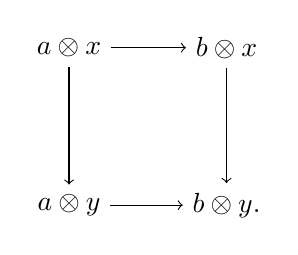
\begin{tikzpicture}
                \node (1) at (0, 0) {$a\otimes x$};
                \node (2) at (2, 0) {$b\otimes x$};
                \node (3) at (0, -2) {$a\otimes y$};
                \node (4) at (2, -2) {$b\otimes y.$};
                \draw[->] (1) -- (2);
                \draw[->] (1) -- (3);
                \draw[->] (2) -- (4);
                \draw[->] (3) -- (4);
            \end{tikzpicture}
        \end{gather*}
        The dual concept (where one of the arguments is contravariant) is sometimes called a \textbf{pullback-hom}, \textbf{pullback-exponential} or \textbf{pullback-power} depending on which bifunctor is used in the definition. In fact, the requirement that $\mathbf{M}$ carries a monoidal structure can be dropped and any bifunctor $\func{\circledast}{C\times D}{E}$ can be used. This more general construction is sometimes called the \textbf{Leibniz construction} and the case where the bifunctor is a tensor bifunctor is then called the \textbf{Leibniz tensor}.
    }

    \newdef{Quillen bifunctor}{\index{Quillen!bifunctor}
        Any bifunctor satisfying the pushout-product axiom that preserves colimits in both variables is called a \textbf{(left) Quillen bifunctor}. It should be noted that the tensor product automatically satisfies this last property in the case of closed monoidal categories.

        In fact, the natural setting for defining Quillen bifunctors is that of two-variable adjunctions \ref{cat:two_variable_adjunction}. Consider such a triple of bifunctors $(\otimes,\mathrm{hom}_L,\mathrm{hom}_R)$.
        \begin{itemize}
            \item The bifunctor $\func{-\otimes-}{C\times D}{E}$ is said to be \textbf{left Quillen} if its pushout-product of cofibrations is again a cofibration and if the acyclicity of any of the domain morphisms implies the acyclicity of the result.
            \item The bifunctors $\mathrm{hom}_L:\mathbf{C}^{op}\times\mathbf{E}\rightarrow\mathbf{D}$ and $\mathrm{hom}_R:\mathbf{D}^{op}\times\mathbf{E}\rightarrow\mathbf{C}$ are said to be \textbf{right Quillen} if the Leibniz product of a cofibration and a fibration is a fibration and if the acyclicity of any of the domain morphisms implies the acyclicity of the result.
        \end{itemize}
        It can be shown that if one of these bifunctors is Quillen, the other two are also Quillen.
    }
    \remark{The fact that in the two-variable adjunction approach one does not mention preservation of (co)limits follows from the property that left (resp. right) adjoints preserve colimits (resp. limits).}

    \newdef{Monoidal model category}{\index{monoidal!model category}
        A model category $\mathbf{M}$ that carries the structure of a closed symmetric monoidal category $(\mathbf{M},\otimes,\mathbf{1})$ such that the following compatibility conditions are satisfied:
        \begin{enumerate}
            \item\textbf{Pushout-product}: The tensor bifunctor and internal homs define a Quillen two-variable adjunction.
            \item\textbf{Unit}: For every cofibrant object $x$ and every cofibrant replacement $\mathbf{1}^{\mathrm{c}}$ of $\mathbf{1}$, the induced morphism $\mathbf{1}^{\mathrm{c}}\otimes x\rightarrow x$ is a weak equivalence.
        \end{enumerate}
    }

    \newdef{Enriched model category}{\index{category!enriched}\index{Joyal-Tierney calculus}
        Let $\mathcal{V}$ be a monoidal model category. A category $\mathbf{M}$ is called a $\mathcal{V}$-enriched model category if is satisfies the following conditions:
        \begin{enumerate}
            \item $\mathbf{M}$ is a $\mathcal{V}$-enriched category that is both powered and copowered over $\mathcal{V}$.
            \item The underlying category $\mathbf{M}_0$ is a model category.
            \item The copower is a left Quillen bifunctor or, equivalently, the power is a right Quillen bifunctor.
        \end{enumerate}
    }
    \begin{example}[Simplicial model category]\label{model:simplicial_model_category}
        A model category enriched over the standard model category of simplicial sets $\mathbf{sSet}_{Quillen}$. It can be shown that the full subcategory of a simplicial model category on fibrant-cofibrant objects is enriched over Kan-complexes.
    \end{example}

\subsection{Homotopy category}\label{section:homotopy_category}

    \newdef{Homotopy}{\index{homotopy}
        Before being able to construct homotopies in general model categories, thereby generalizing the ideas from Section \ref{section:homotopy}, one has to define the counterpart of the unit interval in a model category $\mathbf{C}$. To this end consider an object $x\in\ob{C}$. By taking the product and coproduct of two copies of $x$, one can construct the unique diagonal and codiagonal morphisms $\Delta:x\rightarrow x\times x$ and $\nabla:x\sqcup x\rightarrow x$. By factorizing these morphisms in $\mathbf{C}$, two weak equivalences are obtained:
        \begin{gather}
            x\rightarrow\mathrm{Path}(x),\\
            \mathrm{Cyl}(x)\rightarrow x.
        \end{gather}
        These objects are called the \textbf{path object} and \textbf{cylinder object} respectively. By choosing the morphism to be a fibration (resp. cofibration), the notion of \textbf{good} cylinder (resp. path) object is obtained.

        Using these objects one can define left and right homotopies between parallel morphisms $f,g:x\rightarrow y$. A left homotopy between $f$ and $g$ is a morphism $\eta:\mathrm{Cyl}(x)\rightarrow y$ such that Diagram \ref{fig:left_homotopy} commutes. Analogously, a right homotopy between $f$ and $g$ is a morphism $\lambda:x\rightarrow\mathrm{Path}(y)$ such that Diagram \ref{fig:right_homotopy} commutes. The existence of homotopies induces an equivalence relation on morphisms.

        \begin{figure}
            \centering
            \begin{subfigure}[b]{0.49\textwidth}
                \centering
                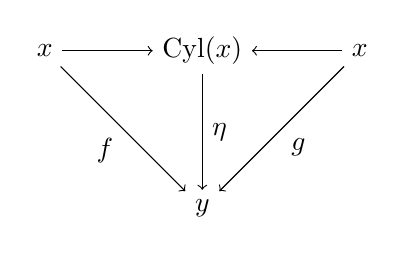
\begin{tikzpicture}
                    \node (X) at (-2,0) {$x$};
                    \node (X2) at (2,0) {$x$};
                    \node (C) at (0,0) {$\mathrm{Cyl}(x)$};
                    \node (Y) at (0,-2) {$y$};
                    \draw[->] (X) -- (C);
                    \draw[->] (X2) -- (C);
                    \draw[->] (C) -- node[right]{$\eta$} (Y);
                    \draw[->] (X) -- node[below left]{$f$} (Y);
                    \draw[->] (X2) -- node[below right]{$g$} (Y);
                \end{tikzpicture}
                \caption{A left homotopy.}
                \label{fig:left_homotopy}
            \end{subfigure}
            \begin{subfigure}[b]{0.49\textwidth}
                \centering
                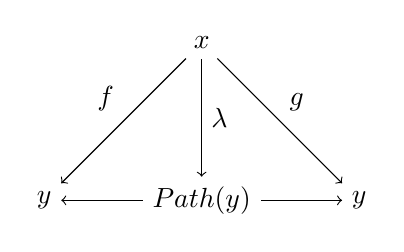
\begin{tikzpicture}
                    \node (Y) at (-2,-2) {$y$};
                    \node (Y2) at (2,-2) {$y$};
                    \node (C) at (0,-2) {$\text{Path}(y)$};
                    \node (X) at (0,0) {$x$};
                    \draw[<-] (Y) -- (C);
                    \draw[<-] (Y2) -- (C);
                    \draw[<-] (C) -- node[right]{$\lambda$} (X);
                    \draw[<-] (Y) -- node[above left]{$f$} (X);
                    \draw[<-] (Y2) -- node[above right]{$g$} (X);
                \end{tikzpicture}
                \caption{A right homotopy.}
                \label{fig:right_homotopy}
            \end{subfigure}
            \caption{Homotopies in a model category.}
        \end{figure}
    }

    \begin{example}[Topological spaces]
        Consider the category $\mathbf{Top}$. A cylinder object $\mathrm{Cyl}(X)$ for a topological space $X$ is given by the product $X\times[0,1]$. The codiagonal map is factorized as the endpoint inclusion $X\sqcup X\rightrightarrows X\times[0,1]$ followed by the collapse $X\times[0,1]\overset{\pi_X}{\rightarrow}X$, where it is not hard to show that the collapse is a homotopy equivalence. A left homotopy with respect to $X\times[0,1]$ is exactly a homotopy in the sense of Definition \ref{topology:homotopy}.

        A path object $\mathrm{Path}(X)$ is given by the mapping space $X^{[0,1]}$. The diagonal map is factorized by the basepoint inclusion $X\overset{\iota_0}{\rightarrow}X^{[0,1]}$ followed by the endpoint projections $X^{[0,1]}\rightrightarrows X\times X$. That the right homotopies with respect to $X^{[0,1]}$ give the same equivalence classes as the left homotopies is the content of Property \ref{topology:path_space}.
    \end{example}

    \begin{property}
        If $x$ is cofibrant, every left homotopy induces a right homotopy. Dually, if $y$ is fibrant, every right homotopy induces a left homotopy.
    \end{property}
    \begin{result}
        Whenever $x$ is cofibrant and $y$ is fibrant, the relations of being left homotopic (or equivalently right homotopic) coincide on $\mathbf{C}(x,y)$ and, in particular, define equivalence relations. The equivalence classes are denoted by $[x,y]$.
    \end{result}

    \begin{property}[Stability under composition]
        Homotopies are preserved under both precomposition and postcomposition by arbitrary morphisms.
    \end{property}
    \begin{property}[Weak equivalences]
        A morphism is a weak equivalence if and only if it is a homotopy inverse.
    \end{property}

    \newdef{Homotopy equivalence}{\index{homotopy!equivalence}
        Two objects in a model category are said to be homotopy equivalent if there exists morphisms $f:x\leftrightarrows y:g$ such that $f\circ g$ and $g\circ f$ are homotopic to the identity. The morphisms $f,g$ are then said to be homotopy equivalences.
    }

    In Definition \ref{model:localization} it was shown that one can assign to every category with weak equivalences a ``homotopy category''. When the category has the additional structure of a model category, one can construct an equivalent category:
    \newadef{Homotopy category I}{\index{homotopy!category}\label{model:homotopy_category_2}
        Let $\mathbf{C}$ be a model category. The homotopy category $\mathbf{Ho}(\mathbf{C})$ is the category defined by the following data:
        \begin{itemize}
            \item\textbf{Objects}: $\ob{C}$
            \item\textbf{Morphisms}: $[x^{\mathrm{cf}},y^{\mathrm{cf}}]$
        \end{itemize}
    }
    In fact it is easier to restrict to the subcategory $\mathbf{C_{cf}}$ of $\mathbf{Ho(C)}$ on the fibrant-cofibrant objects due to the following property (when restricting to a subcategory, the resulting homotopy category is only equivalent and not isomorphic to the localization):
    \begin{property}
        The homotopy category of a model category is equivalent to those of the full subcategories on (co)fibrant objects:
        \begin{gather}
            \mathbf{Ho(C)}\cong\mathbf{Ho(C_f)}\cong\mathbf{Ho(C_c)}\cong\mathbf{Ho(C_{cf})}.
        \end{gather}
    \end{property}

    \begin{theorem}[Whitehead]\index{Whitehead}
        A weak equivalence between objects that are both fibrant and cofibrant is a homotopy equivalence.
    \end{theorem}

    \begin{property}
        A Quillen equivalence between model categories induces an equivalence of homotopy categories.
    \end{property}

    \begin{property}[Monoidal model categories]
        The homotopy category of a monoidal model category has a closed monoidal structure defined by the induced derived adjunction. The homotopy category of an enriched model category is the underlying category of a category enriched, powered and copowered over the homotopy category of its enriching category, where the enriched structure is again given by the induced derived adjunction.
    \end{property}

    In some cases it is useful to consider categories that are strictly weaker than model categories but stronger than categories with weak equivalences. The prime example being the full subcategories of a model category on the (co)fibrant objects. These are often easier to handle in the setting of homotopy theory. To formalize this notion, the following definition is introduced:
    \newdef{Category of fibrant objects}{\index{fibrant object}\index{fibration}
        A category $\mathbf{C}$ with weak equivalences $\mathbf{W}\hookrightarrow\mathbf{C}$ equipped with another subcategory $\mathbf{F}\hookrightarrow\mathbf{C}$ for which the morphisms are called \textbf{fibrations} such that the following conditions are satisfied:
        \begin{enumerate}
            \item $\mathbf{C}$ admits finite products.
            \item Fibrations and acyclic fibrations are preserved under arbitrary pullbacks.
            \item Every object admits a \textbf{good path object}, i.e.~a factorization of the product map $x\rightarrow x\times x$ as the composition of a weak equivalence and a fibration.
            \item All objects are \textbf{fibrant}, i.e.~the terminal map $x\rightarrow1$ is a fibration for all objects $x\in\ob{C}$.
        \end{enumerate}
    }

    \begin{theorem}[Factorization lemma]\index{factorization!lemma}
        Let $\mathbf{C}$ be a category of fibrant objects. Any morphism $f:x\rightarrow y$ can be factorized as the right inverse of an acyclic fibration followed by a fibration.
    \end{theorem}

    The following theorem is important for characterizing functors that preserve weak equivalences:
    \begin{theorem}[Ken Brown's lemma]\index{Ken Brown}\label{model:ken_brown}
        Let $\mathbf{A}$ be a category of fibrant objects and let $\mathbf{B}$ be a category with weak equivalences. If a functor $\func{F}{A}{B}$ maps acyclic fibrations to weak equivalences, it preserves all weak equivalences.
    \end{theorem}
    \remark{An analogous theorem exists for categories of cofibrant objects.}

    The above lemma allows to define derived functors for Quillen functors between model categories (the following definition is also better suited for working in the $\infty$-setting than Definition \ref{model:derived_functor}):
    \newadef{Derived functor}{\index{derived!functor}\label{model:derived_functor_replacement}
        Let $\func{F}{A}{B}$ be a left (resp. right) Quillen functor. The left (resp. right) derived functors are obtained by precomposition with the cofibrant (resp. fibrant) replacement functors.
    }
    \begin{property}[Derived functors are absolute]\label{model:absolute_derived_functors}
        It can be shown that derived functors built using (co)fibrant replacement are given by absolute Kan extensions. So, even though homotopy categories often do not admit all (co)limits, the resulting Kan extensions do exist.
    \end{property}

\subsection{Reedy model structure}

    Consider a complete and cocomplete category $\mathbf{M}$ (in the remainder of this section this will often be $\mathbf{sSet}$). For any full subcategory inclusion $\mathbf{B}\hookrightarrow\mathbf{A}$ one obtains an induced \textbf{truncation} (or \textbf{restriction}) functor $\tr:\mathbf{M^A}\rightarrow\mathbf{M^B}$. The left and right adjoints of this functor are respectively called the \textbf{skeleton} and \textbf{coskeleton} functors.
    \begin{formula}
        The adjoint functors are defined by Kan extensions and hence we can express them in terms of (co)ends and weighted (co)limits:
        \begin{gather}
            \mathrm{sk}(X)x := \int^{y\in\mathbf{B}}\mathbf{A}(y,x)\cdot Xy = \colim^{\mathbf{A}(-,x)}\\
            \mathrm{cosk}(X)x := \int_{y\in\mathbf{B}}[\mathbf{A}(x,y),Xy] = \wlim{\mathbf{A}(x,-)}X.
        \end{gather}
    \end{formula}
    \newdef{Skeletal sets}{\index{skeleton}
        Let $\mathbf{M}=\mathbf{sSet}$ and consider the inclusion $\simplex_{\leq n}\hookrightarrow\simplex$ of the full subcategory on the objects $\{[0],\ldots,[n]\}$. The $n$-truncation functor $\tr_n$ discards all simplices of degree higher than $n$ or, in other words, it ``truncates'' a simplicial set at degree $n$.

        The $n$-skeleton functor $\mathrm{sk}_n$ takes a simplicial set $X$ of degree $\leq n$ and freely adds degenerate simplices in degrees $>n$, i.e.~it is the smallest simplicial set containing $X$ as a simplicial subset. The $n$-coskeleton functor $\mathrm{cosk}_n$ adds a simplex in degree $>n$ whenever all of its faces are present, i.e.~the $m$-simplices in $\text{cosk}_nX$ are given by the collection of all $(m+1)$-tuples of $(m-1)$-simplices that are compatible (along lower simplices).
    }
    \begin{property}[Simplicial nerve]\index{nerve}
        The nerve functor $\func{N}{Cat}{sSet}$ from Sefinition \ref{model:nerve} is a fully faithful functor to the category of 2-coskeletal simplicial sets. This follows from the fact that in ordinary categories, compositions of morphisms are unique and, hence, all higher-order tuples of composable morphisms are determined by composable pairs. In fact, this is just the characterization of (small) categories as categories internal to $\mathbf{Set}$ (under the isomorphism $C_2\cong C_1\times_{C_0}C_1$ which will be called the first \textit{Segal condition} in Definition \ref{model:segal_space}).
    \end{property}

    \newdef{Reedy category}{\index{Reedy category}\label{model:reedy}
        A category $\mathbf{C}$ equipped with a \textbf{degree} function $\ob{C}\rightarrow\alpha$, where $\alpha$ is an ordinal \ref{set:ordinal}, and two wide subcategories $\mathbf{C}^\pm$ that satisfy the following conditions:
        \begin{enumerate}
            \item Nontrivial morphisms in $\mathbf{C}^+$ (strictly) increase the degree.
            \item Nontrivial morphisms in $\mathbf{C}^-$ (strictly) decrease the degree.
            \item All morphisms admit a unique factorization as a morphism in $\mathbf{C}^-$ followed by a morphism in $\mathbf{C}^+$. This factorization is sometimes called the \textbf{(canonical) Reedy factorization}.
        \end{enumerate}
    }

    \begin{property}[Minimality]\index{degree!of factorization}
        The Reedy factorization is the (unique) factorization of minimal degree, where the \textbf{degree} of a factorization $x\overset{f}{\rightarrow}y\overset{g}{\rightarrow}z$ is defined as the degree of $y$.
    \end{property}
    \begin{property}[Isomorphisms are trivial]
        A morphism in a Reedy category is an isomorphism if and only if it is trivial.
    \end{property}

    \begin{example}
        Some common examples of Reedy categories are discrete categories, finite posets, the simplex category $\simplex$ and opposites of Reedy categories.
    \end{example}

    For Reedy categories one can also define $n$-truncation, $n$-skeleton and $n$-coskeleton functors by restricting to the full subcategories on elements of degree $\leq n$.
    \newdef{Matching and latching objects}{\index{matching!object}\index{latching object}
        Let $\mathbf{R}$ be a Reedy category and consider a diagram $X\in\funccat{R}{C}$ with $\mathbf{C}$ small. Consider the skeleton monad and coskeleton comonads (often just called the skeleton and coskeleton functors) $\mathbf{sk}_n:=\mathrm{sk}_n\circ\tr_n$ and $\mathbf{cosk}_n:=\mathrm{cosk}_n\circ\tr_n$. The latching and matching objects of $X$ are defined as the restrictions of $\mathbf{sk}_{n-1}$ and $\mathbf{cosk}_{n-1}$ to the degree $n$ subcategory of $\mathbf{R}$. The counit of the skeleton adjunction and the unit of the coskeleton adjunction give rise to the \textbf{latching} and \textbf{matching} maps.

        One can also define the latching and matching objects through (co)limits. Define the subcategory $\mathbf{R}^+(r)$ as the subcategory of $\mathbf{R}^+/r$ on all objects except the identity. The latching object $L_rX$ can be shown to be isomorphic to the colimit of $X$ over $\mathbf{R}^+(r)$.
    }

    \begin{example}[Simplicial objects]\index{Eilenberg-Zilber}
        The above property allows to give a nice interpretation to latching objects in the case of $\mathbf{R}=\simplex^{op}$. Using the \textit{Eilenberg-Zilber lemma} it can be shown that the $n^{th}$ latching object of a simplicial object is given by its collection of degenerate $n$-simplices.
    \end{example}

    \newdef{Boundary}{\index{boundary}
        The boundary of a representable presheaf $\mathbf{R}(-,r)$ is defined as the latching object of the Yoneda embedding $\func{\mathcal{Y}}{R}{Psh(R)}$ at $r$. It is denoted by $\partial\mathbf{R}(-,r)$. It can be shown that $\partial\mathbf{R}(-,r)$ consists of exactly those morphisms that are not in $\mathbf{R}^-$ or, equivalently, as $\mathbf{sk}_{n-1}\mathbf{R}(-,r)$. The latching map coincides with the canonical inclusion $\partial\mathbf{R}(-,r)\hookrightarrow\mathbf{R}(-,r)$ if $r$ is of degree $n$.
    }
    \begin{formula}
        One can show that the latching and matching objects can be obtained through (co)limits weighted by boundaries:
        \begin{align}
            M_rX &\cong \wlim{\partial\mathbf{R}(r,-)}X\\
            L_rX &\cong \colim^{\partial\mathbf{R}(-,r)}X.\label{model:latching_boundary}
        \end{align}
    \end{formula}

    From here on $\mathbf{M}$ will be assumed to be a model category. In this case a canonical model structure on the functor category $\funccat{R}{M}$ for Reedy $R$ can be defined.
    \newdef{Relative matching and latching objects}{
        Consider the (weighted) colimit bifunctor $\func{\text{colim}}{Psh(R)\times[R,M]}{M}$. The Leibniz construction \ref{model:pushout_product} allows to define the relative latching object of $f:X\rightarrow Y$ at $r\in\ob{R}$ as the Leibniz product of the boundary inclusion $\partial\mathbf{R}(-,r)\hookrightarrow\mathbf{R}(-,r)$ and $f$.

        By Equations \eqref{cat:weighted_hom_colimit} and \eqref{model:latching_boundary}, the relative latching map is of the form $Xr\sqcup_{L_rX}L_rY\rightarrow Yr$ and the relative matching map is of the form $Xr\rightarrow Yr\times_{M_rY}M_rX$.
    }

    \begin{property}[Reedy model structure]
        Let $\mathbf{R}$ be a Reedy category and let $\mathbf{M}$ be a model category. The functor category $\funccat{R}{M}$ admits the following model structure:
        \begin{itemize}
            \item\textbf{Weak equivalences}: the objectwise weak equivalences.
            \item\textbf{Fibrations}: morphisms for which the relative matching map is a fibration (in $\mathbf{M}$) for all $r\in\ob{R}$
            \item\textbf{Cofibrations}: morphisms for which the relative latching map is a cofibration (in $\mathbf{M}$) for all $r\in\ob{R}$
        \end{itemize}
    \end{property}

    \begin{property}[Quillen (co)limit functors]
        Consider a $\mathcal{V}$-enriched model category $\mathbf{M}$ and a Reedy category $\mathbf{R}$. For every Reedy cofibrant functor $W$ in $\funccat{R}{\mathcal{V}}$, the weighted limit and colimit functors are right and left Quillen, respectively.
    \end{property}

    ?? COMPLETE (this section is way too abstract and difficult at this point) ??

\section{Simplicial spaces}
\subsection{Kan complexes}

    \newdef{Horn}{\index{horn}
        Consider the standard simplex $\Delta[n]$. For all $n\geq1$ and $0\leq k\leq n$ the $(n,k)$-horn $\Lambda^k[n]$ is defined as the subsimplicial set obtained by removing the $k^{th}$ face from $\partial\Delta[n]$. When $k=0$ or $k=n$, the horn is said to be \textbf{outer}, otherwise it is said to be \textbf{inner}.
    }

    \newdef{Kan fibration}{\index{Kan!fibration}
        A morphism of simplicial sets that has the right lifting property with respect to all horn inclusions $\Lambda^k[n]\hookrightarrow\Delta[n]$.
    }
    \newdef{Kan complex}{\index{Kan!complex}
        \nomenclature[S_Kan]{$\mathbf{Kan}$}{category of Kan complexes}
        A simplicial set that has all horn fillers or, equivalently, a simplicial set for which the terminal morphism is a Kan fibration. The full subcategory of $\mathbf{sSet}$ on Kan complexes is denoted by $\mathbf{Kan}$.
    }

    \begin{property}[Horn filler condition]\label{model:horn_filler}
        A simplicial set is the nerve of a (small) category if and only if all of its inner horns admit a unique filler. If one requires all horns to admit a unique filler, the nerve of a groupoid is obtained.
    \end{property}

    By relaxing the above requirements one can generalize the notion of a category (due to \textit{Boardman} and \textit{Vogt}):
    \newdef{Quasicategory\footnotemark}{\index{quasi-!category}\index{logos}\index{Boardman condition}\label{model:quasicategory}
        \footnotetext{Some authors such as \textit{Joyal} call these \textbf{logoi} (singular: \textbf{logos}).}
        A simplicial set for which all inner horns have (not necessarily unique) fillers. This condition is sometimes called the \textbf{Boardman condition}.
    }

    At this point the first instance of a ``homotopy category'' can be defined:
    \newdef{Homotopy category II}{\index{homotopy!category}
        Let $X$ be a quasicategory. The homotopy category $\mathbf{Ho}(X)$ consists of the following data:
        \begin{itemize}
            \item\textbf{Objects}: $X_0$
            \item\textbf{Morphisms}: The quotient of $X_1$ under the relation $f\circ g\sim h$ if there exists a 2-simplex with edges $f,g$ and $h$.
        \end{itemize}
    }
    \begin{property}[Fundamental category]\index{fundamental!category}
        If $X$ is a quasicategory, its homotopy category is equivalent to its \textbf{fundamental category} $\pi_1(X)$, i.e.~the image under the left adjoint of the (simplicial) nerve functor.
    \end{property}

    The following theorem is a restatement of Property \ref{model:horn_filler}:
    \begin{theorem}[Joyal]\index{Joyal}
        A quasicategory is a Kan complex if and only if its homotopy category is a groupoid.
    \end{theorem}

\subsection{Simplicial localization}

    \newdef{Homotopy category III}{\index{homotopy!category}\label{model:enriched_homotopy_category}
        Consider a simplicially enriched category $\mathbf{C}$. Its homotopy category $\pi_0(\mathbf{C})$ is defined as follows:
        \begin{itemize}
            \item\textbf{Objects}: $\ob{C}$
            \item\textbf{Morphisms}: $\pi_0\mathbf{C}(x,y)$
        \end{itemize}
        Two morphism $f,g\in\mathbf{C}(x,y)$ are said to be \textbf{homotopic} if they are identified in $\pi_0(\mathbf{C})$. A morphism $f\in\mathbf{C}(x,y)$ is called a \textbf{homotopy equivalence} if it admits both a left and a right inverse in $\pi_0(\mathbf{C})$, i.e.~if it becomes an isomorphism in the homotopy category.
    }
    \newdef{Dwyer-Kan equivalence I}{\index{equivalence!Dwyer-Kan}\label{model:enriched_dwyer_kan}
        Consider a simplicial functor $\func{F}{C}{D}$ between two simplicially enriched categories. This functor is called a Dwyer-Kan equivalence if:
        \begin{itemize}
            \item $F$ is \textbf{$\infty$-fully faithful}, i.e.~the induced map on hom-objects is a weak equivalence. \footnote{This is a generalization of the ordinary definition for categories. (Simplicial categories will give models for $\infty$-categories.)}
            \item The induced map on connected components $\pi_0( F):\pi_0(\mathbf{C})\rightarrow\pi_0(\mathbf{D})$ is an equivalence (of categories). In fact, this condition can be relaxed to $\pi_0F$ being essentially surjective, since together with the previous condition this implies that $\pi_0F$ is an equivalence.
        \end{itemize}
    }

    \begin{construct}[Hammock localization]\index{localization!hammock}
        Let $(\mathbf{C},W)$ be a category with weak equivalences. Its hammock localization (or \textbf{simplicial localization}) $L^H\mathbf{C}$ is the simplicially enriched category constructed as follows:
        \begin{itemize}
            \item\textbf{Objects}: $\ob{C}$
            \item\textbf{Morphisms}: $L^H\mathbf{C}(x,y)$ is the simplicial set defined as follows:
            \begin{quote}
                First, for every $n\in\mathbb{N}$ one constructs a category with as objects the zigzags of morphisms in $\mathbf{C}$ relating $x$ and $y$ such that all left-pointing morphisms are in $W$, and as morphisms the endpoint-preserving ``natural transformations'' (in the sense that all triangles/squares in the resulting diagram commute). Then, the coproduct is taken over the (simplicial) nerves of the categories for all $n\in\mathbb{N}$. Finally, the quotient is taken by the equivalence relations generated by:
                \begin{enumerate}
                    \item inserting or removing identity morphisms, and
                    \item composing composable morphisms.
                \end{enumerate}
            \end{quote}
        \end{itemize}
    \end{construct}

    \begin{property}
        Let $(\mathbf{C},W)$ be a category with weak equivalences. It can be shown that
        \begin{gather}
            \mathrm{Ho}(L^H\mathbf{C})\cong\mathbf{C}[W^{-1}].
        \end{gather}
        This construction gives a more explicit description of the homotopy category. Furthermore, if $\mathbf{M}$ is a simplicial model category, the categories $\mathbf{M_{cf}}$ and $L^H\mathbf{M}$ are Dwyer-Kan equivalent.
    \end{property}
    \begin{property}
        Quillen equivalent model categories have Dwyer-Kan equivalent simplicial localizations.
    \end{property}
    \begin{property}
        Up to Dwyer-Kan equivalence, every simplicially enriched category can be obtained as the simplicial localization of a category with weak equivalences.
    \end{property}

    \newdef{Simplicial resolution}{\index{resolution!(co)simplicial}
        Consider an object $x$ in a model category $\mathbf{M}$. A (co)simplicial resolution of $x$ is a Reedy (co)fibrant (co)simplicial object $X$ together with a weak equivalence $x\simeq X_0$.

        Every object in a model category admits a (co)simplicial resolution by taking a (co)fibrant replacement of the constant (co)simplicial object.
    }

    \newdef{Bergner model structure}{\index{Bergner model structure}
        The catgory of simplicially enriched categories admits the following model structure:
        \begin{itemize}
            \item\textbf{Weak equivalences}: Dwyer-Kan equivalences
            \item\textbf{Cofibrant objects}: \textit{simplicial computads}
            \item\textbf{Fibrant objects}: $\mathbf{Kan}$-enriched categories
        \end{itemize}
    }
    \newconstr{Free resolution}{\index{resolution}\label{model:bergner_free_resolution}
        Consider a (small) category $\mathbf{C}$. From this category we can construct a simplicial category $\mathfrak{C}\mathbf{C}$ consisting of the following data:
        \begin{itemize}
            \item\textbf{Objects}: $\ob{C}$
            \item\textbf{Morphisms}: $\text{hom}(\mathfrak{C}\mathbf{C})_n := \text{hom}(F^{n+1}\mathbf{C})$, where $F$ is identity-on-objects and $F\mathbf{C}$ has as morphisms strings of composable morphisms in $\mathbf{C}$
        \end{itemize}
        It can be shown that $\mathfrak{C}\mathbf{C}$ is a \textit{simplicial computad} for any simplicially enriched category $\mathbf{C}$, $\mathfrak{C}$ acts as the cofibrant replacement functor in the Bergner model structure.
    }

\subsection{Segal spaces}

    \begin{example}[Bisimplicial sets]
        One can also look at simplicial objects in $\mathbf{sSet}$ (these are in particular $\mathbf{sSet}$-enriched). Such objects are often called bisimplicial sets or \textbf{simplicial spaces}\footnote{The latter name follows from the fact that topological spaces and simplicial sets are (Quillen-)equivalent.}. Since $\mathbf{sSet}$ is a model category, Property \ref{model:model_functor_category} above says that $\mathbf{ssSet}$ itself admits a model structure. It can furthermore be shown that the injective model structure on $\mathbf{ssSet}$ coincides with the Reedy model structure (a rather nontrivial statement).
    \end{example}

    \newdef{Segal space}{\index{Segal!space}\index{spine}\label{model:segal_space}
        Consider a fibrant object $X$ in the injective (or Reedy) model structure on $\mathbf{ssSet}$. This bisimplicial set is called a Segal space if it satisfies the following weak form of the \textit{Segal condition} for all $n\geq1$:\footnote{If the Reedy condition is omitted, the limit on the right-hand side has to be replaced by a \textit{homotopy limit}.}
        \begin{gather}
            X_n\simeq X_1\times_{X_0}\cdots\times_{X_0}X_1\ \ (n\text{ factors}).
        \end{gather}
        These maps are called \textbf{Segal maps} (even when they are not weak equivalences). They are the morphisms induced by \textbf{spine} inclusions, i.e.~inclusions of the union of edge 1-cells.
    }
    \newdef{Segal category}{\index{Segal!category}
        A bisimplicial set $X$ is called a \textbf{Segal precategory} if $X_0$ is discrete. It is called a Segal category if in addition all its Segal maps are weak equivalences, i.e.~if it is a Segal space with a discrete set of ``objects''.
    }

    \newdef{Mapping space}{\index{mapping!space}
        Consider a Segal space $X$. For every two points $x,y\in X_0$, the mapping space $\mathrm{Map}(x,y)$ is defined as the fibre of $(d_1,d_0):X_1\rightrightarrows X_0\times X_0$ over the point $(x,y)$. The identity element for $x\in X_0$ is given by $s_0(x)$.
    }

    The following two definitions should be compared to definitions \ref{model:enriched_homotopy_category} and \ref{model:enriched_dwyer_kan}:
    \newdef{Homotopy category IV}{\index{homotopy!category}
        Consider a Segal category $X$. Its homotopy category $\mathbf{Ho}(X)$ is defined as follows:
        \begin{itemize}
            \item\textbf{Objects}: $X_0$
            \item\textbf{Morphisms}: $\pi_0\mathrm{Map}(x,y)$
        \end{itemize}
        Two points $f,g\in\mathrm{Map}(x,y)$ are said to be \textbf{homotopic} if they are identified in $\mathbf{Ho}(X)$. A point $f\in\mathrm{Map}(x,y)$ is called a \textbf{homotopy equivalence} if it admits both a left and a right inverse in $\mathbf{Ho}(X)$, i.e.~if it becomes an isomorphism. The subspace $X_{\mathrm{hoequiv}}\subset X_1$ consists of the components that contain homotopy equivalences.\footnote{It should be noted that if any point in a component is a homotopy equivalence, all points in that component are homotopy equivalences.}
    }
    \newdef{Dwyer-Kan equivalence II}{\index{equivalence!Dwyer-Kan}
        A map $F$ of Segal spaces such that:
        \begin{enumerate}
            \item the induced map on mapping spaces is a weak equivalence.
            \item the induced map between homotopy categories is an equivalence (of categories).
        \end{enumerate}
    }

    \newdef{Complete Segal space}{
        A Segal space $X$ for which the map $s_0:X_0\rightarrow X_{\mathrm{hoequiv}}$ is a weak equivalence.
    }
    \begin{property}[Dwyer-Kan equivalence]
        A map of Segal spaces is a Dwyer-Kan equivalence if and only if it is a weak equivalence in the \textit{complete Segal space model structure}. A map of complete Segal spaces is a Dwyer-Kan equivalence if and only if it is a levelwise weak equivalence.
    \end{property}

\subsection{Coherent nerve}

    The nerve and realization functors \ref{model:nerve_and_realization} can also be modified to incorporate the higher homotopical data present in a simplicially enriched category.

    First, define a cosimplicial simplicially enriched category $\func{C}{\Delta}{sSetCat}$ that assigns to every finite ordinal $[n]$ the category consisting of the following data:
    \begin{itemize}
        \item\textbf{Objects}: $[n]\equiv\{0,1,\ldots,n\}$
        \item\textbf{Morphisms}: $C[n](i,j) := N(P_{ij})$, where $N$ is the ordinary nerve functor on $\mathbf{Cat}$ and $P_{ij}$ is the poset consisting of all subsets of $\{i,\ldots,j\}$ that contain both $i$ and $j$.
    \end{itemize}
    The (homotopy) \textbf{coherent nerve functor} (or \textbf{simplicial nerve functor}\footnote{This terminology was also used for the ordinary nerve functor taking values in $\mathbf{sSet}$. In general it should be clear from the context which one is meant.}) is the nerve functor induced by this cosimplicial object. It not only knowns about all possible morphisms, it also knows about all possible ways how one can obtain this morphism.
    \begin{remark}
        The cosimplicial object $\func{C}{\Delta}{sSetCat}$ is in fact just the free resolution functor $\mathfrak{C}$ in the Bergner model structure \ref{model:bergner_free_resolution} restricted to the subcategory $\simplex$.
    \end{remark}

    \begin{property}
        The homotopy coherent nerve functor $N_\Delta$ is uniquely determined by the following relation:
        \begin{gather}
            \mathbf{sSet}(\Delta[n],N_\Delta\mathbf{C})=\mathbf{sSetCat}(C[n],\mathbf{C}).
        \end{gather}
    \end{property}

    \begin{property}[Simplicial realization]
        The left adjoint of the homotopy coherent nerve functor satisfies the following relation for all finite ordinals $[n]$:
        \begin{gather}
            |\Delta[n]|\cong C[n].
        \end{gather}
    \end{property}

    \begin{property}[Quasicategories]
        If $\mathbf{C}$ is $\mathbf{Kan}$-enriched, its coherent nerve is a quasicategory. By Example \ref{model:simplicial_model_category} this allows to associate a quasicategory to any simplicial model category by passing to the coherent nerve of its fibrant-cofibrant subcategory.
    \end{property}

    At this point it is interesting to reconsider the simplicial nerve construction \ref{model:nerve}. Although the functor $\func{N}{Cat}{sSet}$ is fully faithfull, there is a problem in that weak equivalences of simplicial sets do not necessarily correspond to (weak) equivalences of categories. The issue comes from the definition of the canonical model structure \ref{model:sset_model_structure} on $\mathbf{sSet}$. Here, the weak equivalences are those morphisms that become weak equivalences after geometric realization. During this step information about the direction of morphisms is lost and it becomes impossible to distinguish categories from groupoids. Only when all morphisms are assumed to be invertible, i.e.~the category is assumed to be groupoid, does one recover the converse statement.

    A first solution is to use a different model structure with less weak equivalences:
    \newdef{Joyal model structure}{\index{Joyal!model structure}
        The category $\mathbf{sSet}$ of simplicial sets \ref{model:simplicial set} admits a model structure defined by the following data:
        \begin{itemize}
            \item\textbf{Weak equivalences}: \textit{weak categorical equivalences}, i.e.~maps $f:X\rightarrow Y$ such that the induced simplicial functor $C(f):C(X)\rightarrow C(Y)$ is a Dwyer-Kan equivalence.
            \item\textbf{Cofibrations}: monomorphisms
            \item\textbf{Fibrant objects}: quasicategories \ref{model:quasicategory}
        \end{itemize}
    }
    When characterizing those simplicial sets that are nerves of categories, groupoids and categories are distinguished by whether all horns admit a (unique) filler or only inner horns admit a (unique) filler. However, when the fibrant objects are Kan complexes (those simplicial sets that admit all horn fillers), the homotopical structure only knows about nerves that come from a groupoid. By passing to the larger class of quasicategories, this problem is solved.

    Instead of changing the model structure on $\mathbf{sSet}$ to overcome the issues with taking nerves of categories or groupoids, one can also change the construction of the nerve functor. An alternative approach was introduced by \textit{Rezk}:
    \newdef{Classifying diagram}{\index{classifying!diagram}
        Consider a (small) category $\mathbf{C}$ together with the functor category $\mathbf{C}^{[n]}$ where $[n]$ is the totally ordered set on $n+1$ elements. The classifying diagram of $\mathbf{C}$ is the bisimplicial set $\widetilde{N}\mathbf{C}$ defined levelwise as follows:
        \begin{gather}
            \widetilde{N}\mathbf{C}_k := N(\text{Core}(\mathbf{C})),
        \end{gather}
        where $N$ is the ordinary nerve functor and $\mathrm{Core}$ denotes the core functor \ref{cat:core}.

        The reason for why this construction is better for distinguishing categories and groupoids comes from the fact that information about isomorphisms is already captured at degree 0, while information about noninvertible morphisms is only captured from degree 1 onwards.
    }
    \begin{property}
        If $\mathbf{C}$ is small, then $\widetilde{N}\mathbf{C}$ is a complete Segal space.
    \end{property}

    ?? COMPLETE ??

\section{Cofibrant generation}
\subsection{Transfinite constructions}

    Before proceeding, some notions from ordinary category need to be specialized to the context of regular cardinals \ref{set:regular_cardinal}. In this section the symbol $\kappa$ will always denote such a regular cardinal.

    \newdef{$\kappa$-filtered category}{\index{category!filtered}
        A category in which every diagram with less than $\kappa$ arrows admits a cocone.
    }
    \newdef{$\kappa$-directed limit}{\index{limit!directed}
        Consider a poset $I$ such that every subposet of cardinality less than $\kappa$ has a lower bound (upper bound for directed colimits). Such a set is said to be $\kappa$-(co)directed. A limit of a diagram over this poset is called a $\kappa$-(co)directed (co)limit.
    }
    The following definition is a categorification of the previous one:
    \newdef{$\kappa$-filtered limit}{\index{limit!filtered}
        Consider a diagram $\func{D}{I}{C}$. The limit (resp. colimit) of $D$ is said to be $\kappa$-cofiltered (resp. $\kappa$-filtered) if $\mathbf{I}$ is a $\kappa$-cofiltered (resp. $\kappa$-filtered) category.

        It should be noted that an analogue of Property \ref{cat:directed_filtered} also holds in the $\kappa$-context, i.e.~a category has all $\kappa$-directed colimits if and only if it has all $\kappa$-filtered colimits (and analogously for limits).
    }

    \newdef{Small object}{\index{small}\index{presentable}
        An object for which there exists a regular cardinal $\kappa$ such that its covariant hom-functor preserves all $\kappa$-filtered colimits. These objects are also said to be \textbf{$\kappa$-compact} or \textbf{$\kappa$-presentable}.
    }
    \newdef{Accessible category}{\index{accessible}
        A locally small category $\mathbf{C}$ for which there exists a regular cardinal $\kappa$ such that $\mathbf{C}$ has all $\kappa$-filtered colimits and such that $\mathbf{C}$ contains a small subcategory $\mathbf{D}$ of $\kappa$-small objects that generates all objects by $\kappa$-filtered colimits, i.e.~$\mathbf{C}\cong\mathrm{Ind}_\kappa(\mathbf{D})$.
    }
    \newdef{Locally presentable category}{\index{presentable}
        A cocomplete, accessible category. It can be shown that such categories are also complete and, hence, bicomplete.
    }

    \begin{property}
        Every locally presentable category can be obtained as a full reflective subcategory of a presheaf category under an \textbf{accessible embedding}, i.e.~an embedding that preserves filtered colimits.
    \end{property}
    \begin{property}[Gabriel-Ulmer duality]\index{Gabriel-Ulmer duality}
        There exists an equivalence between locally finitely presentable categories and categories of left exact copresheaves from small complete categories. This gives a 2-equivalence $\mathbf{Lex}^{op}\cong\mathbf{LFP}$.
    \end{property}

    \begin{theorem}[Adjoint functor theorem]\index{adjoint functor theorem}
        Consider a functor $\func{F}{C}{D}$ between locally presentable categories. $F$ admits a right adjoint if and only if it preserves all colimits. $F$ admits a left adjoint if and only if it is accessible and if it preserves all limits.
    \end{theorem}

    For ordinary categories the axioms guarantee the existence of a (unique) composition of any finite number of (composable) morphisms. However, in some cases it is useful, or even necessary, to talk about the ``composite'' of an infinite number of morphisms:
    \newdef{Transfinite composition}{\index{composition}\label{cat:transfinite_composition}
        Consider a category $\mathbf{C}$ with a collection of morphisms $I\subseteq\mathrm{hom}(\mathbf{C})$ and let $\alpha$ be an infinite ordinal \ref{set:ordinal}. A ($\alpha$-indexed) \textbf{transfinite sequence} of morphisms in $I$ is a diagram of the form $\func{D}{\alpha}{C}$ such that:
        \begin{enumerate}
            \item Successor morphisms in $\alpha$ are mapped to elements of $I$.
            \item $D$ is \textit{continuous} in the sense that for every limit ordinal $\beta<\alpha$: $D\beta\cong\underset{\gamma<\beta}{\colim}\ D\gamma$.
        \end{enumerate}
        $D\lambda$ denotes the restriction of $D$ to the (full) subdiagram $\{\gamma\mid\gamma<\lambda\}$ of $\alpha$. The transfinite composition of this sequence is the induced morphism $D_0\rightarrow D\alpha\equiv\colim\ D$.
    }
    \newdef{Cell complex}{\index{cell!complex}
        Consider a cocomplete category $\mathbf{C}$ with a collection of morphisms $I\subseteq\mathrm{hom}(\mathbf{C})$. A \textbf{relative} $I$-cell complex is a transfinite composition of pushouts (of coproducts\footnote{It can be shown that closure under coproducts follows automatically.}) of morphisms in $I$. An $I$-cell complex is an object such that the unique morphism from the initial object is a relative $I$-cell complex.
    }
    \newnot{Relative cell complexes}{
        The set of all relative $I$-cell complexes is often denoted by $\mathrm{cell}(I)$.
    }

\subsection{Cofibrant generation}

    The following is a famous result by \textit{Quillen}:
    \begin{theorem}[Small object argument]\index{small!object argument}
        Let $\mathbf{C}$ be a locally presentable category with a collection of morphisms $I\subseteq\mathrm{hom}(\mathbf{C})$. Every morphism in $\mathbf{C}$ can be factorized as the composition of a morphism in $\mathrm{rlp}(I)$ followed by a morphism in $\mathrm{cell}(I)$.
    \end{theorem}
    \begin{remark}
        This theorem can be generalized to cocomplete categories where the morphisms in $I$ are small relative\footnote{\textit{Small relative to a set of morphisms} is defined just as ordinary smallness, but with general $\kappa$-filtered colimits replaced by those that start from morphisms in the given set.} to $\mathrm{cell}(I)$. Sets of morphisms with this property are said to \textbf{admit a small object argument}.
    \end{remark}

    \newdef{Cofibrantly generated model category}{\index{model!category}
        Consider a model category $\mathbf{C}$. This category is said to be cofibrantly generated by two sets of morphisms $I,J\subseteq\mathrm{hom}(\mathbf{C})$ if it satisfies the following conditions:
        \begin{enumerate}
            \item $I$ and $J$ both admit the small object argument.
            \item The fibrations are given by $\mathrm{rlp}(J)$.
            \item The acyclic fibrations are given by $\mathrm{rlp}(I)$.
        \end{enumerate}
        It can be shown that the last two conditions are equivalent to the following ones:
        \begin{enumerate}
            \item[$2^*.$] The cofibrations are the retracts (in the arrow category) of $\mathrm{cell}(I)$.
            \item[$3^*.$] The acyclic fibrations are the retracts (in the arrow category) of $\mathrm{cell}(J)$.
        \end{enumerate}
        The morphisms in $I$ and $J$ are called the \textbf{generating cofibrations} and \textbf{generating acyclic cofibrations}, respectively.
    }

    Sometimes it is desirable to replace the model structure on a category $\mathbf{C}$ by one that has more weak equivalences (denote the new one by $\mathbf{C}_0$). If the cofibrations remain the same, this new structure has some nice properties:
    \begin{itemize}
        \item The fibrations are a subclass of the original ones.
        \item The acyclic fibrations remain the same.
        \item The identity functors $\mathrm{Id}:\mathbf{C}_0\leftrightarrows\mathbf{C}:\mathrm{Id}$ form a Quillen adjunction.
        \item Every object in $\mathbf{C}$ is weakly equivalent (in $\mathbf{C}_0$) to one in $\mathbf{C}_0$.
    \end{itemize}

    This procedure can be made explicit for a specific class of model categories. Let $\mathbf{C}$ be a left proper, cofibrantly generated, simplicial model category and consider a collection $S\subset\mathrm{hom}(\mathbf{C})$ of cofibrations with cofibrant domain. First, the notion of ``$S$-local objects'' is introduced:
    \newdef{Local object}{\index{local!object}
        A fibrant object $x$ is said to be $S$-local if for all morphisms in $S$ the image under the Yoneda embedding of $x$ is an acyclic Kan fibration. Analogously, a morphism is called an $S$-local weak equivalence if for all $S$-local fibrant objects its image under their Yoneda embeddings is an acyclic Kan fibration.
    }
    \begin{property}
        Every weak equivalence is an $S$-local weak equivalence: $W\subset W_S$.
    \end{property}

    \begin{construct}[Left Bousfield localization]\index{localization!Bousfield}
        Given a model category $\mathbf{C}$ with the same assumptions as before, the (left) Bousfield localization $L_S\mathbf{C}$ is defined as as the same category but with the following model structure:
        \begin{itemize}
            \item\textbf{Cofibrations}: $\mathrm{cof}(\mathbf{C})$
            \item\textbf{Acyclic cofibrations}: cofibrations that are $S$-local weak equivalences
        \end{itemize}
        If it exists, the Bousfield localization $L_S\mathbf{M}$ of $\mathbf{M}$ at $S$ is the universal left Quillen functor $\gamma:\mathbf{M}\rightarrow L_S\mathbf{M}$ such that its left derived functor sends the image of $S$ to isomorphisms in $\mathbf{Ho}(\mathbf{M})$. The identity functor gives a Quillen adjunction between $\mathbf{M}$ and $L_S\mathbf{M}$ and the induced adjunction on homotopy categories defines a reflective localization.
    \end{construct}
    \begin{remark}
        The notions of local object/morphisms can be slightly generalized (they give equivalent localizations). A \textbf{$S$-local morphism} $f:a\rightarrow b$ is a morphism such that for all objects $x\in\ob{M}$ for which the map
        \begin{gather}
            \mathbf{M}(g^\mathrm{c},x^\mathrm{f}):\mathbf{M}(d^\mathrm{c},x^\mathrm{f})\rightarrow\mathbf{M}(c^\mathrm{c},x^\mathrm{f})
        \end{gather}
        is a weak equivalence for all $g\in S$ ($x$ is said to be \textbf{$S$-local}), the map
        \begin{gather}
            \mathbf{M}(f^\mathrm{c},x^\mathrm{f}):\mathbf{M}(b^\mathrm{c},x^\mathrm{f})\rightarrow\mathbf{M}(a^\mathrm{c},x^\mathrm{f})
        \end{gather}
        is also a weak equivalence. This is the homotopical version of Definition \ref{cat:local_object}, after cofibrant (resp. fibrant) replacement of the domain (resp. codomain), the Yoneda embedding of every $S$-local object is weak equivalence, where $S$-local objects are those objects whose Yoneda embedding maps morphisms in $S$ to weak equivalences.
    \end{remark}

    \newdef{Combinatorial model category}{
        A locally presentable, cofibrantly generated model category.
    }

    \begin{theorem}[Dugger]\index{Dugger}\label{model:dugger}
        Every combinatorial model category is Quillen equivalent to a (left) Bousfield localization of a category of simplicial presheaves on a small category (with the global projective model structure).
    \end{theorem}

    ?? FINISH ??

\section{Homotopy (co)limits}

    Consider a category $\mathbf{C}$ with weak equivalences together with diagrams $\func{D,D'}{I}{C}$. Assume that there exists a weak equivalence between $D$ and $D'$, i.e.~a natural transformation that consists of componentwise weak equivalences. Clearly this induces a morphism between (co)limits, but it would be nice if the construction of (co)limits would also preserve the homotopical structure, i.e.~weakly equivalent diagrams should have weakly equivalent (co)limits.

    The main purpose of this section is to introduce a modification of the ordinary (co)limit functors that takes into account the homotopical structure of the underlying categories.

    A first step is the modification of (co)products:
    \newdef{Homotopy (co)products}{\index{homotopy!(co)product}
        In ordinary categories the universal property of a product (and dually for coproducts) characterizes it as an object with an isomorphism
        \begin{gather}
            \mathbf{C}(-,c)\cong\prod_{i\in I}\mathbf{C}(-,c_i)
        \end{gather}
        such that every $I$-indexed collection of morphisms $f_i:x\rightarrow c_i$ can be factorized as follows
        \begin{gather*}
            \begin{tikzpicture}
                \node (X) at (-1, 1) {$x$};
                \node (C) at (-1, -1) {$c$};
                \node (CI) at (1, -1) {$c_i.$};
                \draw[->] (X) -- node[above right]{$f_i$} (CI);
                \draw[->] (C) -- node[below]{$\pi_i$} (CI);
                \draw[->, dashed] (X) -- node[left]{$\exists!$} (C);
            \end{tikzpicture}
        \end{gather*}
        To obtain a homotopical version, the commutativity of this diagram is relaxed up to a homotopy/path in the hom-space $\mathbf{M}(x,c_i)$. This leads to the definition of a homotopy product as an object $c$ together with a natural weak (homotopy) equivalence
        \begin{gather}
            \psi_x:\mathbf{C}(x,c)\simeq\prod_{i\in I}\mathbf{C}(x,c_i).
        \end{gather}
        The homotopy (co)products are unusual in the sense that they can be obtained as (co)limits in the homotopy category $\mathbf{Ho(C)}$.
    }

    More generally, one can define homotopy (co)limits in any homotopical category by passing to derived functors:
    \newdef{Homotopy (co)limits}{\index{homotopy!(co)limits}
        Let $\mathbf{A}$ be a homotopical category and let $\mathbf{B}$ be a small category. The homotopy limit and colimit functors are defined as the derived functors of the limit and colimit functors $\mathrm{(co)lim}:\funccat{B}{A}\rightarrow\mathbf{A}$.
    }
    \begin{remark}
        The reason for why (co)products can be obtained as ordinary (co)limits  is related to the fact that their indexing categories are discrete. In this case the adjoint of the derived functor is equivalent to the diagonal functor on the homotopy category.
    \end{remark}

    \begin{property}[Model categories]
        Consider the specific case where $\mathbf{C}$ is a model category. If $\funccat{D}{C}$ admits an injective (resp. projective) model structure, the homotopy limit (resp. colimit) always exists and can be obtained through fibrant (resp. cofibrant) replacement as in Definition \ref{model:derived_functor_replacement}.
    \end{property}
    \begin{example}[Reedy categories]
        Consider the general case of diagrams $\func{D}{R}{C}$ with $\mathbf{R}$ Reedy. First, note that the constant functor $\func{\Delta}{C}{[R,C]}$ maps weak equivalences to (pointwise) weak equivalences.\footnote{This is also true when $\mathbf{R}$ is not Reedy.} If the Reedy structure is such that the constant functor preserves cofibrations, then this functor is left Quillen and Ken Brown's lemma \ref{model:ken_brown} implies that its right Quillen adjoint, the limit functor, preserves weak equivalences. In this case one can define the \textbf{homotopy limit} $\mathrm{holim}\,D$ as the functor $\lim(D\circ Q_\mathrm{f})$, where $Q_\mathrm{f}$ is the fibrant replacement-functor (which in this case acts pointwise). A dual construction gives rise to \textbf{homotopy colimits}.
    \end{example}

\subsection{Simplicially enriched diagrams}

    In the setting where diagrams are enriched over $\mathbf{sSet}$, one can define homotopy (co)limits in a more sophisticated way.

    \newdef{Homotopy colimit}{
        Consider a diagram $\func{D}{I}{C}$ with $\mathbf{C}$ copowered over $\mathbf{sSet}$. The homotopy colimit of $D$ is defined as the following tensor product \ref{cat:copower_product}:
        \begin{gather}
            \mathrm{hocolim}\,D := N(-/\mathbf{I})\otimes_\mathbf{I}D = \int^{i\in\mathbf{I}}N(i/\mathbf{I})\cdot Di,
        \end{gather}
        where $N$ is the nerve functor \ref{model:nerve}.
    }
    A similar definition for homotopy limits can be used when the category is powered over $\mathbf{sSet}$:
    \newdef{Homotopy limit}{
        Consider a diagram $\func{D}{I}{C}$ with $\mathbf{C}$ powered over $\mathbf{sSet}$. The homotopy limit of $D$ is defined as the following hom-like object:
        \begin{gather}
            \mathrm{holim}\,D := \int_{i\in\mathbf{I}}[N(\mathbf{I}/i),Di].
        \end{gather}
        This is exactly the characterization of the homotopy limit as the $\mathbf{sSet}$-natural transformations between $N(\mathbf{I}/-)$ and $D$.
    }
    \begin{remark}[Bousfield-Kan map]\index{Bousfield-Kan map}
        The expressions from the above formulas are also known as the \textbf{Bousfield-Kan formulas}. It should be noted that the above definitions are not strictly equivalent to the ones from the previous section. To be precise, the Bousfield-Kan formulas are only weakly equivalent to the general definitions if the objects in $\mathbf{C}$ are replaced by their (co)fibrant replacements, i.e.~if in the above expressions $D$ is postcomposed by a (co)fibrant replacement-functor.
    \end{remark}

    ?? COMPLETE (CHECK THESE STATEMENTS) ??

    By Definition \ref{model:homotopy_category_2} one can construct morphisms in a homotopy category as morphisms from a cofibrant replacement to a fibrant replacement. This allows to define diagrams-up-to-homotopy (in two settings):
    \newdef{Homotopy coherent diagram}{\index{homotopy!diagram}
        A morphism in the homotopy category of the Bergner model category. When considering diagrams taking values in a $\mathbf{Kan}$-enriched category, one can use the free resolution functor to characterize them as functors $D:\mathfrak{C}\mathbf{I}\rightarrow\mathbf{C}$. Since the simplicial realization functor extends the free resolution functor $\mathfrak{C}$ to simplicial sets, one can also define homotopy coherent diagrams on simplicial sets.

        Natural transformations between such diagrams are given by homotopy coherent diagrams $\mathfrak{C}(\mathbf{I}\times\Delta[1])\rightarrow\mathbf{C}$ in analogy with ordinary homotopies. However, these do no compose uniquely in the sense that one does not obtain a well-defined diagram on $\mathbf{I}\times\Delta[2]$. Therefore, one does not obtain a category of homotopy coherent diagrams. For simplicial sets $I$ it can be shown that the natural structure is that of a quasicategory:
        \begin{gather}
            \mathbf{CohDgrm(I,C)}\cong(N\mathbf{C})^\mathbf{I},
        \end{gather}
        where $N$ is the simplicial nerve functor.
    }

    ?? COMPLETE ??

\section{\texorpdfstring{$\infty$-categories}{Infinity-categories}}
\subsection{Simplicial approach}

    The first approach to $\infty$-category theory is the simplicial one. The motivation is Property \ref{model:horn_filler}, which relates the categorical structure to the existence of certain horn fillers. The generalization is then given by the notion of quasicategories \ref{model:quasicategory}.

    \begin{theorem}[Lurie]\index{Lurie}\label{model:lurie_presentation}
        An $\infty$-category is presentable if and only if it is equivalent to  the coherent nerve of the fibrant-cofibrant subcategory of a combinatorial model category and, hence by Dugger's theorem \ref{model:dugger}, can be presented by simplicial presheaves.
     \end{theorem}